\makeatletter\def\input@path{{images/}{styles/}{corps/}{bib/}}\makeatother

\documentclass{transp_java}
\usepackage{colortbl}
%\usepackage{ulem}
\title[Langage et algorithmique]{Langage et algorithmique \\ \textcolor[rgb]{0.5,0,0.5}{- Arbre -}}
\author{A. Malek TOUMI\\ toumiab@ensta-bretagne.fr}
%\date[05/04/2015]{Toumi A. Malek.  Python 3.4}
\date{2015/2016}
\institute{ENSTA Bretagne}


%\usetheme{Transp}
\usetheme{progressbar}
%\usetheme{Darmstadt}
\progressbaroptions{imagename= python-HE.png}



\mode<handout>{
  \usecolortheme{dove}
  \usepackage{pgfpages}
  \pgfpagesuselayout{4 on 1}[a4paper, border shrink=5mm, landscape]
}



\begin{document}

\frame{\titlepage}

\AtBeginSection[]
{
  \begin{frame}<beamer>
    \frametitle{Sommaire}
    \tableofcontents[current,currentsection]
  \end{frame}
}

\AtBeginSubsection[]
{
  \begin{frame}<beamer>
    \frametitle{Sommaire}
    \tableofcontents[current,currentsubsection]
  \end{frame}
}

\newlength\dunder
\settowidth{\dunder}{\_}
\newcommand{\twound}{\rule{2\dunder}{0.4pt}}


%%%


\section{Diff�rents arbres}


\subsection{D�finitions}

\begin{frame}
  \frametitle{Pourquoi des arbres ?}

  \begin{itemize}
  \item<1-> Structure dynamique : liste
  \item<2-> Constat : co�t �lev� des op�rations de base
  \item<3-> Objectif : trouver une structure de donn�es plus efficace
  \end{itemize}

  \uncover<4->{Arbre~:}
  \begin{itemize}
  \item<5-> Structure de donn�es dynamique
  \item<6-> Bonne complexit� pour les op�rations de base
  \item<7-> Recherche, insertion, suppression : $\Theta(\log n)$
  \end{itemize}
\end{frame}

\begin{frame}
  \frametitle{D�finitions}

  \only<1,3,5,7,9,11>{
    \begin{defi}[Arbre]
      Ensemble non vide de noeuds et d'ar�tes tel que~:
      \begin{itemize}[<+->]
      \item<3-> noeud : objet simple
      \item<5-> ar�te : relie deux noeuds (orient�)
      \item<7-> branche : suite de noeuds reli�s par des ar�tes
      \item<9-> racine : noeud sans pr�d�cesseur
      \item<11-> tous les noeuds sont accessibles depuis la racine par une
        seule branche
      \end{itemize}
    \end{defi}}
  
  \begin{center}
    \only<2,4,6,8,10>{
\begin{tikzpicture}
  \tikzstyle{noeud}=[circle, draw=black, rounded corners, ball
  color=olive!60, text centered, text=black, minimum size=0.5cm]
\only<4>{
  \tikzstyle{noeud}=[circle, draw=black, rounded corners, ball
  color=purple!60, text centered, text=black, minimum size=0.5cm]
}
  \tikzstyle{fleche}=[->,shorten >=1pt,auto,thick]
  \node[noeud] (root) {};
  \node[noeud, below=of root] (na) {};
  \node[noeud, left=of na] (nb) {};
  \node[noeud, right=of na] (nc) {};
  \node[noeud, below=of nb] (nd) {};
  \node[noeud, left=of nd] (ne) {};
  \foreach \a/\b in {root/na,root/nb,root/nc,nb/nd,nb/ne} {
    \draw (\a) -- (\b);
    \only<6>{
      \draw[thick,color=purple] (\a) -- (\b);
    }
  }
  \only<8>{
    \node[noeud, ball color=purple!60] (root) {};
    \node[noeud, left=of na, ball color=purple!60] (nb) {};
    \node[noeud, below=of nb, ball color=purple!60] (nd) {};
      \draw[thick,color=purple] (root) -- (nb);
      \draw[thick,color=purple] (nb) -- (nd);
  }
  \only<10>{
    \node[left=of root] (r) {Racine};
    \draw[fleche] (r) -- (root);
  }
 % \node[right=of nd] (f) {Feuilles};
 % \draw[fleche] (f) -- (nd);
 % \draw[fleche] (f) -- (na);
\end{tikzpicture}
    }
  \end{center}
\end{frame}


\begin{frame}
  \frametitle{D�finitions}

  \only<1,3>{
    \begin{itemize}
    \item Repr�sentation : racine au sommet de l'arbre
    \item Relation p�re-fils entre les noeuds
    \item Bas de l'arbre : feuilles
    \end{itemize}
    \uncover<3>{
      \begin{defi}[Hauteur]
        Nombre de noeuds du plus long chemin entre la racine et les feuilles.
      \end{defi}
    }
  }
  \only<2,4>{
    \begin{center}
\begin{tikzpicture}[node distance=1cm]]
  \tikzstyle{noeud}=[circle, draw=black, rounded corners, ball
  color=olive!60, text centered, text=black, minimum size=0.5cm]
  \tikzstyle{fleche}=[->,shorten >=1pt,auto,thick]
  \node[noeud] (root) {};
  \node[noeud, below=of root] (na) {};
  \node[noeud, left=of na] (nb) {};
  \node[noeud, right=of na] (nc) {};
  \node[noeud, below=of nb] (nd) {};
  \node[noeud, left=of nd] (ne) {};
  \foreach \a/\b in {root/na,root/nb,root/nc,nb/nd,nb/ne} {
    \draw (\a) -- (\b);
  }
  \node[left=of root] (r) {Racine};
  \draw[fleche] (r) -- (root);
  \node[right=of nd] (f) {Feuilles};
  \draw[fleche] (f) -- (nd);
  \draw[fleche] (f) -- (na);
  \only<4>{
    \node[right=of nc] (x1) {};
    \node[node distance=1.5cm,above=of x1] (x0) {};
    \node[node distance=1.5cm,below=of x1] (x2) {};
    \draw[thick,<->] (x0) -- node[right] {Hauteur 3} (x2);
  }
\end{tikzpicture}
    \end{center}
  }
\end{frame}


\subsection{Arbres binaires}

\begin{frame}
  \frametitle{D�finition}

  \only<1>{
    \begin{defi}[Arbre binaire]
      Un arbre binaire est un arbre dont chaque noeud poss�de au plus deux
      fils. 
    \end{defi}

    \begin{defi}[Arbre binaire complet]
      Un arbre est complet si chaque noeud qui n'est pas une feuille poss�de
      exactement deux fils et o� toutes les feuilles sont au m�me niveau.
    \end{defi}
  }

  \only<2>{
    \begin{center}
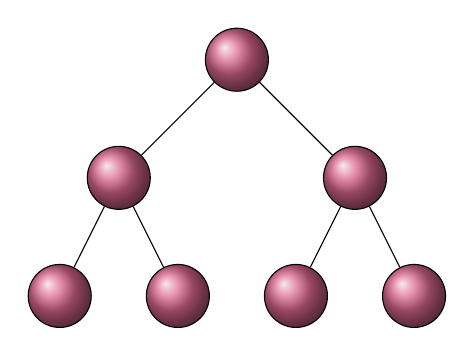
\begin{tikzpicture}[scale=1.5]
  \tikzstyle{noeud}=[circle, draw=black, rounded corners, ball
  color=purple!60, text centered, text=black, minimum size=0.8cm]
  \tikzstyle{fleche}=[->,shorten >=1pt,auto,thick]
  \foreach \n/\x/\y in {r/2.5/3,a/1.5/2,b/3.5/2,c/1/1,d/2/1,e/3/1,f/4/1} {
    \draw (\x,\y) node[noeud] (\n) {};
  }
  \foreach \a/\b in {r/a,r/b,a/c,a/d,b/e,b/f} {
    \draw (\a) -- (\b);
  }
\end{tikzpicture}
%      \includegraphics[height=5cm]{arbreComplet}
    \end{center}
  }
\end{frame}

\begin{frame}
  \frametitle{Propri�t�s}
  \begin{itemize}[<+->]
  \item Chaque noeud poss�de un fils gauche et un fils droit
  \item Arbre de hauteur $h$
  \item[$\Rightarrow$] $2^h-1$ noeuds (si complet)
  \item $n$ noeuds
  \item[$\Rightarrow$] hauteur $\log n$
  \end{itemize}
\end{frame}

\begin{frame}[fragile]
  \frametitle{en Python}
  \lstset{language=Python}
  \begin{block}{Code pour d�finir un noeud}
    \begin{lstlisting}[frame=single,escapechar=\#]
     class Node(object):
         #\visible<2->{#def \_\_init\_\_(self, valeur = 0):#}#
           #\visible<3->{#     self.val = valeur  #}#
           #\visible<4->{#     self.right = None #}#
           #\visible<4->{#     self.left = None#}#
            #\visible<4->{#\textcolor[rgb]{0,0.58,0}{\#     self.height = 0}#}#
         ...
 
     #\visible<5->{#class Arbre(object):#}#
         #\visible<5->{#def \_\_init\_\_(self):#}#
           #\visible<6->{#     self.\_\_root = None  #}#
         ...
    \end{lstlisting}
  \end{block}
\end{frame}

\begin{frame}
  \frametitle{en Python}
  \begin{center}
\begin{tikzpicture}[node distance=1cm]
  \tikzstyle{noeud}=[rectangle, draw=black, rounded corners, ball
  color=teal!60, text centered, text=black, minimum size=1cm, rectangle
  split, rectangle split parts=2, text width=0.7cm]
  \tikzstyle{fleche}=[->,shorten >=1pt,auto,semithick]
  \node [noeud] (a) {~ \nodepart{second}$|$};
  \node[left=of a] (r) {Racine};
  \node[noeud, below left=of a] (b) {\nodepart{second}$|$};
  \node[noeud, below right=of a] (c) {\nodepart{second}$|$};
  \node[noeud, below left=of c] (d) {\nodepart{second}$|$};
  \node[noeud, below right=of c] (e) {\nodepart{second}$|$};
  \node[noeud, below left=of b] (f) {\nodepart{second}$|$};
  \draw[fleche] ([xshift=3mm,yshift=-2mm] a.west) -- (b.north);
  \draw[fleche] ([xshift=-3mm,yshift=-2mm] a.east) -- (c.north);
  \draw[fleche] ([xshift=3mm,yshift=-2mm] c.west) -- (d.north);
  \draw[fleche] ([xshift=-3mm,yshift=-2mm] c.east) -- (e.north);
  \draw[fleche] ([xshift=3mm,yshift=-2mm] b.west) -- (f.north);
  \draw[fleche] (r) -- (a);
\end{tikzpicture}
%    \includegraphics[height=6cm]{arbreBinaire}
  \end{center}
\end{frame}

%\begin{frame}
%  \frametitle{en Java}
%  \only<1-6>{
%\begin{semiverbatim}
%  public class Node \{\pause
%
%  \hspace{1cm}private String value;\pause
%
%  \hspace{1cm}private Node left;  // fils gauche
%
%  \hspace{1cm}private Node right; // fils droit\pause
%
%
%  \hspace{1cm}public Node(String val)  \{\pause
%
%    \hspace{2cm}value = val;\pause
%
%    \hspace{2cm}left = None;
%
%    \hspace{2cm}right = None;
%
%  \hspace{1cm}\}
%
%  \hspace{1cm}...
%
%\}
%\end{semiverbatim}
%  }
%  \only<7>{
%    \begin{center}
%      \includegraphics[height=6cm]{arbreBinaire}
%    \end{center}
%  }
%\end{frame}


\begin{frame}
  \frametitle{G�n�ralisation}
  Arbres \emph{n-aires} : 
  \begin{itemize}[<+->]
  \item chaque noeud poss�de au plus $n$ fils.
  \item En \emph{Python} : chaque noeud poss�de une liste de $n$ fils
  \item Moins utile que les arbres binaires
  \item Exemple d'utilisation : \emph{quadtree}
  \end{itemize}
\end{frame}

\subsection{Arbres g�n�raux}

\begin{frame}
  \frametitle{D�finition}
 
    \begin{defi}[Arbre g�n�ral]
      Arbre pour lequel chaque noeud poss�de un nombre
      quelconque de fils (non born� \emph{a priori}).
    \end{defi}
    
    \begin{exemple}[Exemples d'utilisation]
      \begin{itemize}
      \item Repr�sentation d'une arborescence de r�pertoires
      \item Repr�sentation des possibilit�s pour un jeu
      \end{itemize}
    \end{exemple}
\end{frame}


\begin{frame}[fragile]
  \frametitle{D�finition}

    \begin{block}{Code pour d�finir un noeud}
    \begin{lstlisting}[frame=single,escapechar=\#]
     class Node(object):  
		
         #\visible<1->{#def \_\_init\_\_(self, valeur = 0):#}#
           #\visible<2->{#     self.val = valeur  #}#
           #\visible<3->{#     self.child = None #}#
           #\visible<4>{#     self.brothers = []#}#
           
    \end{lstlisting}
  \end{block}
\end{frame}

 \begin{frame}
  \frametitle{D�finition}
    \begin{center}
\begin{tikzpicture}[node distance=1cm]
  \tikzstyle{noeud}=[rectangle, draw=black, rounded corners, ball
  color=orange!60!red, text centered, text=black, minimum size=1cm, rectangle
  split, rectangle split parts=2, text width=0.7cm]
  \tikzstyle{fleche}=[->,shorten >=1pt,auto,semithick]
  \node [noeud] (a) {~ \nodepart{second}$|$};
  \node[left=of a] (r) {Racine};
  \node[noeud, below left=of a] (b) {\nodepart{second}$|$};
  \node[noeud, below right=of a] (c) {\nodepart{second}$|$};
  \node[noeud, below left=of c] (d) {\nodepart{second}$|$};
  \node[noeud, right=of d] (e) {\nodepart{second}$|$};
  \node[noeud, right=of e] (g) {\nodepart{second}$|$};
  \node[noeud, below left=of b] (f) {\nodepart{second}$|$};
  \draw[fleche] ([xshift=3mm,yshift=-2mm] a.west) -- (b.north);
  \draw[fleche] ([xshift=-3mm,yshift=-2mm] b.east) -- (c.west);
  \draw[fleche] ([xshift=3mm,yshift=-2mm] c.west) -- (d.north);
  \draw[fleche] ([xshift=-3mm,yshift=-2mm] d.east) -- (e.west);
  \draw[fleche] ([xshift=-3mm,yshift=-2mm] e.east) -- (g.west);
  \draw[fleche] ([xshift=3mm,yshift=-2mm] b.west) -- (f.north);
  \draw[fleche] (r) -- (a);
\end{tikzpicture}
%      \includegraphics[height=6cm]{arbreGeneral}
    \end{center}

\end{frame}


\section{Arbres binaires de recherche}


\subsection{D�finition}

\begin{frame}
  \frametitle{D�finition}
  \begin{defi}[Arbre binaire de recherche]
    Arbre binaire v�rifiant la propri�t� : pour tout noeud $n$ de l'arbre,
    tous les noeuds de son sous-arbre  gauche sont inf�rieurs � $n$,
    tous les noeuds de son sous-arbre droit sont sup�rieurs � $n$.
  \end{defi}

  \begin{center}
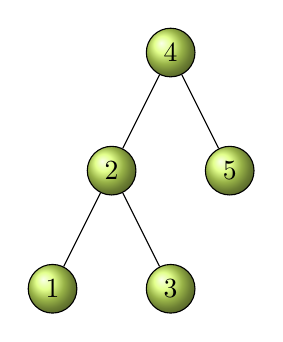
\begin{tikzpicture}[scale=1.5]
  \tikzstyle{noeud}=[circle, draw=black, rounded corners, ball
  color=lime!60, text centered, text=black, minimum size=0.5cm]
  \tikzstyle{fleche}=[->,shorten >=1pt,auto,thick]
  \foreach \n/\x/\y in {1/1/1,2/1.5/2,3/2/1,4/2/3,5/2.5/2} {
    \draw (\x,\y) node[noeud] (\n) {\n};
  }
  \foreach \a/\b in {4/2,4/5,2/1,2/3} {
    \draw (\a) -- (\b);
  }
\end{tikzpicture}
%    \includegraphics[height=4cm]{abr}
  \end{center}
\end{frame}

\subsection{Recherche}

\begin{frame}
  \frametitle{Recherche}
  Rechercher un �l�ment~:
  \begin{itemize}[<+->]
  \item partir de la racine
  \item comparer la valeur recherch�e � l'�l�ment courant
    \begin{itemize}
    \item si elle est �gale : fin
    \item si elle est inf�rieure : chercher dans le sous-arbre gauche
    \item sinon : chercher dans le sous-arbre droit
    \end{itemize}
  \end{itemize}
\end{frame}

\begin{frame}
  \frametitle{Exemple}
  \begin{center}
    \begin{tikzpicture}[scale=2]
      \tikzstyle{noeud}=[circle, draw=black, rounded corners, ball
      color=lime!60, text centered, text=black, minimum size=0.5cm]
      \tikzstyle{fleche}=[->,shorten >=1pt,auto,thick]
      \foreach \n/\x/\y in {1/1/1,2/1.5/2,3/2/1,4/2/3,5/2.5/2} {
        \draw (\x,\y) node[noeud] (\n) {\n};
      }
      \only<2>{\draw (2,3) node[noeud,ball color=red!40] (4) {4};}
      \only<3>{\draw (1.5,2) node[noeud,ball color=red!40] (2) {2};}
      \only<4>{\draw (2,1) node[noeud,ball color=red!40] (3) {3};}
      \foreach \a/\b in {4/2,4/5,2/1,2/3} {
        \draw (\a) -- (\b);
      }
      \draw (3,1) node {Recherche~: 3};
    \end{tikzpicture}
  \end{center}
\end{frame}


\begin{frame}
  \frametitle{Complexit�}
  \only<1-4,6>{
    �tude de l'algorithme~:
    \begin{itemize}[<+->]
    \item pire des cas : aller jusqu'� une feuille
    \item complexit� hauteur de l'arbre
    \item[$\Rightarrow$] arbre complet : $\Theta(\log n)$
    \item arbre le pire : peigne
    \item complexit� : $\Theta(n)$
    \end{itemize}}
  \only<5>{
    \begin{center}
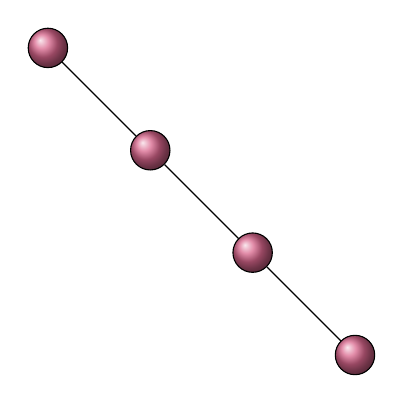
\begin{tikzpicture}[scale=1.3]
  \tikzstyle{noeud}=[circle, draw=black, rounded corners, ball
  color=purple!60, text centered, text=black, minimum size=0.5cm]
  \tikzstyle{fleche}=[->,shorten >=1pt,auto,thick]
  \foreach \n/\x in {a/1,b/2,c/3,d/4} {
    \draw (\x,-\x) node[noeud] (\n) {};
  }
  \foreach \a/\b in {a/b,b/c,c/d} {
    \draw (\a) -- (\b);
  }
\end{tikzpicture}
%      \includegraphics[height=5cm]{peigne}
    \end{center}
  }

\end{frame}

\begin{frame}[fragile]
  \frametitle{Algorithme it�ratif}
\begin{algorithm2e}[H]
  \caption{Recherche it�rative dans un ABR}
%  \label{alg:rechABRi}
  \KwIn{entier val}
%  \KwData{ racine : noeud \tcp{ racine de l'arbre}}
%  \KwData{ n : noeud \tcp{ noeud courant}}
  $n \gets racine$\;
  \While{$n \neq None$ et $n.val \neq val$} {
    \eIf{$val < n.val$} {
      $n \gets n.filsGauche$\;
    }
    {
      $n \gets n.filsDroit$\;
    }
  }
  retourner $n$ \tcp{ n a la valeur recherch�e ou n vaut \emph{None}}
\end{algorithm2e}
  % \begin{algorithmic}[1]
  %   \Procedure{rechIter}{entier val}
  %     \State $n \gets racine$
  %     \While{$n \neq None$ et $n.val \neq val$}
  %       \If{$val < n.val$}
  %         \State $n \gets n.filsGauche$
  %       \Else
  %         \State $n \gets n.filsDroit$
  %       \EndIf
  %     \EndWhile
  %     \State retourner $n$ \Comment n a la valeur recherch�e ou n vaut \emph{None}
  %   \EndProcedure
  % \end{algorithmic}
\end{frame}


\begin{frame}[fragile]
  \frametitle{Algorithme r�cursif}

 \begin{function}[H]
  \caption{rechRec(entier val, Noeud cour)}
  \label{alg:rechABRr2}
  \uIf{$cour = None$ ou $cour.val = val$} {
    retourner cour\;
  }
  \uElseIf{$val < cour.val$} {
    retourner rechRec(val, n.filsGauche)\;
  }
  \Else {
    retourner rechRec(val, n.filsDroit)\;
  }
\end{function}
 % \begin{algorithmic}[1]
 %    \Procedure{rechRec}{entier val, Noeud cour}
 %      \If{$cour = None$ ou $cour.val = val$}
 %        \State retourner cour
 %      \ElsIf{$val < cour.val$}
 %        \State retourner $rechRec(val, n.filsGauche)$
 %      \Else
 %        \State retourner $rechRec(val, n.filsDroit)$
 %      \EndIf
 %    \EndProcedure
 %  \end{algorithmic}
\end{frame}


\subsection{Parcours exhaustif}

\begin{frame}
  \frametitle{Principe}
  \begin{itemize}[<+->]
  \item parcourir un arbre : appliquer un traitement � tous les noeuds
  \item algorithme it�ratif : difficile � �crire
  \item algorithme r�cursif : tr�s simple
    \begin{itemize}
    \item principe~: 3 traitements $\Rightarrow$ 2 sous-arbres et noeud courant
    \item noeud courant avant le fils gauche $\Rightarrow$ pr�fixe
    \item noeud courant entre les fils  $\Rightarrow$ infixe
    \item noeud courant apr�s le fils droit $\Rightarrow$ postfixe
    \end{itemize}
  \end{itemize}
\end{frame}


\begin{frame}
  \frametitle{Exemple : parcours infixe}

\begin{center}
\pgfdeclarelayer{background}
\pgfdeclarelayer{foreground}
\pgfsetlayers{background,main,foreground}
\begin{tikzpicture}[scale=2]
  \tikzstyle{noeud}=[circle, draw=black, rounded corners, ball
  color=cyan!60, text centered, text=black, minimum size=0.5cm]
  \tikzstyle{fleche}=[->,shorten >=1pt,auto,thick]
  \foreach \n/\x/\y in {1/1/1,2/1.5/2,3/2/1,4/2/3,5/2.5/2} {
    \draw (\x,\y) node[noeud] (\n) {\n};
  }
  \foreach \a/\b in {4/2,4/5,2/1,2/3} {
    \draw (\a) -- (\b);
  }
  \only<3>{\draw (2,3) node[noeud,ball color=purple!30!orange] (4) {4};}
  \only<6>{\draw (1,1) node[noeud,ball color=purple!30!orange] (1) {1};}
  \only<7>{\draw (1.5,2) node[noeud,ball color=purple!30!orange] (2) {2};}
  \only<8>{\draw (2,1) node[noeud,ball color=purple!30!orange] (3) {3};}
  \only<2>{
    \begin{pgfonlayer}{background}
      \path (1.west |- 2.north)+(-0.1,0.1) node (a) {};
      \path (3.south -| 3.east)+(+0.1,-0.1) node (b) {};
      \path[fill=yellow!40,rounded corners, draw=black!50, dashed] (a) rectangle (b);
    \end{pgfonlayer}
  }
  \only<4>{
    \begin{pgfonlayer}{background}
      \path (5.west |- 5.north)+(-0.1,0.1) node (a) {};
      \path (5.south -| 5.east)+(+0.1,-0.1) node (b) {};
      \path[fill=yellow!40,rounded corners, draw=black!50, dashed] (a) rectangle (b);
    \end{pgfonlayer}
  }
  \only<5->{
    \begin{pgfonlayer}{background}
      \path (1.west |- 2.north)+(-0.1,0.1) node (a) {};
      \path (3.south -| 3.east)+(+0.1,-0.1) node (b) {};
      \path[fill=yellow!10,rounded corners, draw=black!50, dashed] (a) rectangle (b);
    \end{pgfonlayer}
  }
\end{tikzpicture}
\end{center}
\end{frame}

\begin{frame}[fragile]
  \frametitle{Algorithmes}
  \only<2>{
\begin{procedure}[H]
  \caption{prefixe(Noeud cour)}
  \label{alg:prefixe}
  \If{$cour \neq None$} {
    traiter \emph{cour}\;
    prefixe(cour.filsGauche)\;
    prefixe(cour.filsDroit)\;
  }
\end{procedure}
  % \begin{algorithmic}[1]
  %   \Procedure{prefixe}{Noeud cour}
  %     \If{$cour \neq None$}
  %       \State traiter \emph{cour}
  %       \State prefixe(cour.filsGauche)
  %       \State prefixe(cour.filsDroit)
  %     \EndIf
  %   \EndProcedure
  % \end{algorithmic}
  }
  \only<1>{
\begin{procedure}[H]
  \caption{infixe(Noeud cour)}
  \label{alg:infixe}
  \If{$cour \neq None$} {
    infixe(cour.filsGauche)\;
    traiter \emph{cour}\;
    infixe(cour.filsDroit)\;
  }
\end{procedure}
  % \begin{algorithmic}[1]
  %   \Procedure{infixe}{Noeud cour}
  %     \If{$cour \neq None$}
  %       \State infixe(cour.filsGauche)
  %       \State traiter \emph{cour}
  %       \State infixe(cour.filsDroit)
  %     \EndIf
  %   \EndProcedure
  % \end{algorithmic}
  }
  \only<3>{
 \begin{procedure}[H]
  \caption{postfixe(Noeud cour)}
  \label{alg:postfixe}
  \If{$cour \neq None$} {
    postfixe(cour.filsGauche)\;
    postfixe(cour.filsDroit)\;
    traiter \emph{cour}\;
  }
\end{procedure}
 % \begin{algorithmic}[1]
 %    \Procedure{postfixe}{Noeud cour}
 %      \If{$cour \neq None$}
 %        \State postfixe(cour.filsGauche)
 %        \State postfixe(cour.filsDroit)
 %        \State traiter \emph{cour}
 %      \EndIf
 %    \EndProcedure
 %  \end{algorithmic}
  }
\end{frame}

\begin{frame}
  \frametitle{Exemple : parcours infixe}

  \begin{center}
\pgfdeclarelayer{background}
\pgfdeclarelayer{foreground}
\pgfsetlayers{background,main,foreground}
\begin{tikzpicture}[scale=2]
  \tikzstyle{noeud}=[circle, draw=black, rounded corners, ball
  color=cyan!60, text centered, text=black, minimum size=0.5cm]
  \tikzstyle{fleche}=[->,shorten >=1pt,auto,thick]
  \foreach \n/\x/\y in {1/1/1,2/1.5/2,3/2/1,4/2/3,5/2.5/2} {
    \draw (\x,\y) node[noeud] (\n) {\n};
  }
  \foreach \a/\b in {4/2,4/5,2/1,2/3} {
    \draw (\a) -- (\b);
  }
  \only<6>{\draw (2,3) node[noeud,ball color=purple!30!orange] (4) {4};}
  \only<3>{\draw (1,1) node[noeud,ball color=purple!30!orange] (1) {1};}
  \only<4>{\draw (1.5,2) node[noeud,ball color=purple!30!orange] (2) {2};}
  \only<5>{\draw (2,1) node[noeud,ball color=purple!30!orange] (3) {3};}
  \only<7>{\draw (2.5,2) node[noeud,ball color=purple!30!orange] (5) {5};}
  \only<8>{}
  \only<2>{
    \begin{pgfonlayer}{background}
      \path (1.west |- 2.north)+(-0.1,0.1) node (a) {};
      \path (3.south -| 3.east)+(+0.1,-0.1) node (b) {};
      \path[fill=yellow!10,rounded corners, draw=black!50, dashed] (a) rectangle (b);
    \end{pgfonlayer}
  }
\end{tikzpicture}
\uncover<3->{1}
\uncover<4->{2}
\uncover<5->{3}
\uncover<6->{4}
\uncover<7->{5}
  \end{center}
\end{frame}


\subsection{Insertion}

\begin{frame}
  \frametitle{Principe}

  \begin{itemize}
  \item Insertion uniquement sur les feuilles
  \item Principe : 
    \begin{itemize}
    \item se placer sur la bonne feuille (d�placement it�ratif ou r�cursif)
    \item ajouter le fils
    \end{itemize}
  \item principe similaire � l'insertion dans une liste
  \end{itemize}
\end{frame}

\begin{frame}

  \frametitle{Demo}
  \href{https://moodle.ensta-bretagne.fr/mod/resource/view.php?id=14500}{\includegraphics[height=5cm]{images/arbre_ins.png}}
\end{frame}

\begin{frame}[fragile]
  \frametitle{Algorithme}
  \only<1>{
\begin{algorithm2e}[H]
  \caption{Insertion dans un arbre binaire de recherche}
  \label{alg:insertABR}
  \KwIn{noeud val}
  \eIf{$arbre = \emptyset$} {
    $racine \gets val$\;
  } {
    insert(val, racine) \tcp{ins�re val sous la racine}
  }
\end{algorithm2e}
  % \begin{algorithmic}[1]
  %   \Procedure{insert}{noeud val}
  %     \If{$arbre = \emptyset$}
  %       \State $racine \gets val$
  %     \Else
  %       \State insert(val, racine) \Comment ins�re val sous la racine
  %     \EndIf
  %   \EndProcedure
  % \end{algorithmic}
  }
  \only<2>{
\begin{procedure}[H]
  \caption{insert(noeud val,noeud pere)}
  $n \gets pere$\;
  \While{$n \neq None$} {
    $pere \gets n$\;
    \eIf{$val < n$} {
      $n \gets n.filsGauche$\;
    } {
      $n \gets n.filsDroit$\;
    }
  }
  \tcp{ maintenant le fils de \emph{pere} est None}
\end{procedure}
  % \begin{algorithmic}[1]
  %   \Procedure{insert}{noeud val,noeud pere}
  %     \State $n \gets pere$
  %     \While{$n \neq None$}
  %       \State $pere \gets n$
  %       \If{$val < n$}
  %         \State $n \gets n.filsGauche$
  %       \Else
  %         \State $n \gets n.filsDroit$
  %       \EndIf
  %     \EndWhile \Comment maintenant le fils de \emph{pere} est None
  %   \EndProcedure
  % \end{algorithmic}
  }
  \only<3>{
\begin{procedure}[H]
  \caption{insert(noeud val,noeud pere)}
  \tcp{ \ldots{} maintenant le fils de \emph{pere} est None}
  \eIf{$val < pere$} {
    $pere.filsGauche \gets val$\;
  } {
    $pere.filsDroit \gets val$\;
  }
\end{procedure}
  % \begin{algorithmic}[1]
  %   \Procedure{insert}{noeud val,noeud pere}
  %     \State \ldots{}  \Comment maintenant le fils de \emph{pere} est None
  %     \If{$val < pere$}
  %       \State $pere.filsGauche \gets val$
  %     \Else
  %       \State $pere.filsDroit \gets val$
  %     \EndIf
  %   \EndProcedure
  % \end{algorithmic}
  }
\end{frame}


\subsection{Suppression}

\begin{frame}
  \frametitle{Principe}
  \begin{itemize}
  \item se placer au dessus de l'�l�ment � supprimer
  \item remplacer le noeud par le sous-arbre gauche
  \item r�ins�rer le sous-arbre droit
  \end{itemize}
\end{frame}


\begin{frame}
  \frametitle{Exemple}

  \begin{center}
    \begin{tikzpicture}[scale=1.5]
      \tikzstyle{noeud}=[circle, draw=black, rounded corners, ball
      color=yellow!50, text centered, text=black, minimum
      size=0.2cm,font=\scriptsize] 
      \tikzstyle{fleche}=[->,shorten >=1pt,auto,thick]
      \foreach \n/\x/\y in {1/1/1,2/1.5/2,3/2/1,4/2.5/3} {
        \draw (\x,\y) node[noeud] (\n) {\n};
      }
      \only<-3>{
        \foreach \n/\x/\y in {5/2.5/0,6/3/1,7/3.5/0,9/4/1,8/3.5/2} {
          \draw (\x,\y) node[noeud] (\n) {\n};
        }
        \foreach \a/\b in {4/8,8/6,8/9} {
          \draw (\a) -- (\b);
        }
      }
      \only<2,3>{\draw (3.5,2) node[noeud,ball color=red!50] (8) {8};}
      \only<3>{
        \draw (3,1) node[noeud,ball color=blue!50] (6) {6};
        \draw[fleche, double] (6) to (8);
      }
      \only<4->{
        \foreach \n/\x/\y in {6/3.5/2,5/3/1,7/4/1,9/4.5/0} {
          \draw (\x,\y) node[noeud] (\n) {\n};
        }
        \draw (4) -- (6);
      }
      \only<5>{
        \draw[dashed, semithick, bend right, ->, shorten >=1pt] (9) to (6);
      }
      \foreach \a/\b in {4/2,2/1,2/3,6/5,6/7} {
        \draw (\a) -- (\b);
      }
      \only<6>{
        \draw (7) -- (9);
      }
    \end{tikzpicture}
  \end{center}
\end{frame}

\section{Autres arbres}


\subsection{Arbres syntaxiques}

\begin{frame}
  \frametitle{Arbre syntaxique}  
  \only<1>{
    \begin{itemize}
    \item Arbre repr�sentant un phrase 
    \item ou un programme ou une partie d'un programme
    \item exemple : expression arithm�tique
    \item Sert � analyser la phrase/le programme
    \end{itemize}

    Exemple~: $2+3*4-5$
  }
  \only<2>{
    \begin{center}
      \includegraphics[height=5cm]{images/arbre_synt}
    \end{center}
  }
\end{frame}


\subsection{Syst�me de fichiers}

\begin{frame}
  \frametitle{Fichiers}

  \only<1>{
    \begin{itemize}
    \item Repr�sentation sous forme d'arbre g�n�ral
    \item Fichiers : feuilles
    \item R�pertoires : noeuds interm�diaires
    \end{itemize}
  }

  \only<2>{
    \begin{center}
      \includegraphics[height=5cm]{images/arborescence-dossiers}
    \end{center}
  }
\end{frame}

\subsection{Arbres �quilibr�s}

\begin{frame}
  \frametitle{Int�r�t}
  \begin{itemize}
  \item Arbre binaire : efficace si complet
  \item Arbre binaire complet : pas toujours possible
  \item[$\Rightarrow$] notion d'arbre �quilibr�
  \end{itemize}
  \pause
  \begin{defi}[Arbre �quilibr�]
    Arbre binaire est �quilibr� : la diff�rence entre les
    hauteurs des fils gauche et droit de tout noeud ne peut exc�der 1.
  \end{defi}

\end{frame}

\begin{frame}
  \frametitle{Exemple : arbre d�s�quilibr�}

    \begin{center}
      \includegraphics[height=5cm]{images/arbre_desequilibre}
    \end{center}
\end{frame}

\begin{frame}
  \frametitle{�quilibrage d'un arbre}

  \only<1>{
    \begin{center}
      \includegraphics[height=5cm]{images/equilibrage1}
    \end{center}
  }
  \only<2>{
    \begin{center}
      \includegraphics[height=5cm]{images/equilibrage2}
    \end{center}
  }
  \only<3>{
    \begin{center}
      \includegraphics[height=5cm]{images/equilibrage3}
    \end{center}
  }
  \only<4>{
    \begin{center}
      \includegraphics[height=5cm]{images/equilibrage4}
    \end{center}
  }

\end{frame}


\end{document}


%%% Local Variables: 
%%% mode: latex
%%% TeX-master: t
%%% End: 
